\documentclass[journal,twocolumn]{IEEEtran}
\usepackage[utf8]{inputenc}
\usepackage{amssymb}
\usepackage{amsmath}
\usepackage{graphicx}
\providecommand{\brak}[1]{\ensuremath{\left(#1\right)}}
\newcommand*{\permcomb}[4][0mu]{{{}^{#3}\mkern#1#2_{#4}}}
\newcommand*{\perm}[1][-3mu]{\permcomb[#1]{P}}
\newcommand*{\comb}[1][-1mu]{\permcomb[#1]{C}}
\title{Assignment 1(CBSE Class 12)}
\author{NIMMALA AVINASH(CS21BTECH11039)}
\begin{document}

\maketitle

{\Large \textbf{Exercise 13.5 Question 14.}}

\begin{Large}

In a box containing $100$ bulbs.$10$ are defective. The probability that out of a sample of $5$ bulbs ,none are defective is \\

\end{Large}

{\Large \textbf{Solution:}\\}
\begin{Large}
From the given information, the probability of a bulb being defective is
\begin{align}
p = \frac{10}{100} = \frac{1}{10}\\
\end{align}
Defining $X$ as $B \brak{5,\frac{1}{10}}$  the desired probability is\\
\begin{align}
    Pr\brak{X=0} &= \comb{5}{0} \brak{\frac{1}{10}}^{0} \brak{\frac{9}{10}} ^ {5-0}\\
    &= \brak{\frac{9}{10}}^5
\end{align}
\begin{figure}[h]
\centering
    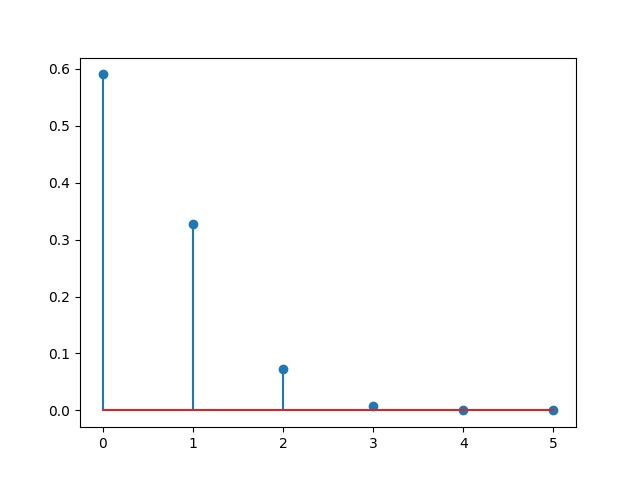
\includegraphics[width = \columnwidth]{Assign_3fig.jpeg}
    \caption{PMF graph}
    \label{fig 1}
\end{figure}
\end{Large}
\end{document}

